\documentclass[12pt,a4paper]{article}
\usepackage{amsmath,amscd,amsbsy,amssymb,latexsym,url,bm,amsthm}
\usepackage{epsfig,graphicx,subfigure}
\usepackage{enumitem,balance}
\usepackage{wrapfig}
\usepackage{mathrsfs,euscript}
\usepackage[usenames]{xcolor}
\usepackage{hyperref}
\usepackage[vlined,ruled,linesnumbered]{algorithm2e}
\usepackage{array}
\hypersetup{colorlinks=true,linkcolor=black}

\newtheorem{theorem}{Theorem}
\newtheorem{lemma}[theorem]{Lemma}
\newtheorem{proposition}[theorem]{Proposition}
\newtheorem{corollary}[theorem]{Corollary}
\newtheorem{exercise}{Exercise}
\newtheorem*{solution}{Solution}
\newtheorem{definition}{Definition}
\theoremstyle{definition}

\renewcommand{\thefootnote}{\fnsymbol{footnote}}

\newcommand{\postscript}[2]
 {\setlength{\epsfxsize}{#2\hsize}
  \centerline{\epsfbox{#1}}}

\renewcommand{\baselinestretch}{1.0}

\setlength{\oddsidemargin}{-0.365in}
\setlength{\evensidemargin}{-0.365in}
\setlength{\topmargin}{-0.3in}
\setlength{\headheight}{0in}
\setlength{\headsep}{0in}
\setlength{\textheight}{10.1in}
\setlength{\textwidth}{7in}
\makeatletter \renewenvironment{proof}[1][Proof] {\par\pushQED{\qed}\normalfont\topsep6\p@\@plus6\p@\relax\trivlist\item[\hskip\labelsep\bfseries#1\@addpunct{.}]\ignorespaces}{\popQED\endtrivlist\@endpefalse} \makeatother
\makeatletter
\renewenvironment{solution}[1][Solution] {\par\pushQED{\qed}\normalfont\topsep6\p@\@plus6\p@\relax\trivlist\item[\hskip\labelsep\bfseries#1\@addpunct{.}]\ignorespaces}{\popQED\endtrivlist\@endpefalse} \makeatother

\usepackage{tikz}
\usepackage{tcolorbox}

\begin{document}
\noindent

%========================================================================
\noindent\framebox[\linewidth]{\shortstack[c]{
\Large{\textbf{Lab08-Graph Exploration}}\vspace{1mm}\\
CS214-Algorithm and Complexity, Xiaofeng Gao \& Lei Wang, Spring 2021.}}
\begin{center}
\footnotesize{\color{red}$*$ If there is any problem, please contact TA Yihao Xie. }

\footnotesize{\color{blue}$*$ Name: Zilong Li  \quad Student ID: 518070910095 \quad Email: logcreative-lzl@sjtu.edu.cn}
\end{center}

\begin{enumerate}

	\item Given an undirected graph $G = (V, E)$. Prove the following propositions.
	
	\begin{enumerate}
		\item Let $e$ be a maximum-weight edge on some cycle of connected graph $G=(V,E)$.
        Then there is a minimum spanning tree of $G$ that does not include $e$. Moreover, there is no minimum spanning tree of $G$ that includes $e$ if $e$ is the unique maximum-weight edge on the cycle. 
		\item Let $T$ and $T'$ are two different minimum spanning trees of $G$. Then $T'$ can be obtained from $T$ by repeatly substitute one edge in $T\backslash T'$ by one edge in $T'\backslash T$ and meanwhile the result after each subsitution is still a minimum spanning tree.
	\end{enumerate}
	
    \item Let $G=(V,E)$ be a connected, undirected graph. Give an $O(|V|+|E|)$-time algorithm
    to compute a path in $G$ that traverses each edge in $E$ exactly once in each direction. Describe how you can find your way out of a maze if you are given enough coins to apply your algorighm.

    \item Consider the maze shown in Figure \ref{Fig-Maze}. The black blocks in the figure are blocks that can not be passed through. Suppose the block are explored in the order of right, down, left and up. That is, to go to the next block from $(X,Y)$, we always explore $(X,Y+1)$ first, and then $(X+1,Y)$,$(X,Y-1)$ and$(X-1,Y)$ at last. Answer the following subquestions:
    \begin{figure}[!htbp]
        \centering
        \includegraphics[width=0.45\textwidth]{Fig-Maze.pdf}
        \caption{The blocks in the maze.}
        \label{Fig-Maze}
    \end{figure}
    \begin{enumerate}
        \item Give the sequence of the blocks explored by using DFS to find a path from the ``start" to the ``finish".
        \begin{solution}
            The DFS order is:
            \begin{tcolorbox}
                AA, AB, BB, CB, CC, CA, DA, EA, EB, EC, ED, DD
            \end{tcolorbox}
            which is shown in Figure \ref{fig:dfs}.

            And the path found is:
            \begin{tcolorbox}
                AA, AB, BB, CB, CA, DA, EA, EB, EC, ED, DD
            \end{tcolorbox}

            \begin{figure}[h]
                \centering
                \begin{tikzpicture}
\tikzstyle{rect}=[minimum width=1cm,minimum height=1cm,draw];
\tikzstyle{block}=[rect,fill=black];
\tikzstyle{visit}=[rect,fill=gray!20];
\draw[help lines]  (-2,1) grid (3,-4);
\node [block] at (-0.5,0.5) {};
\node [block] at (-0.5,-1.5) {};
\node [block] at (0.5,-2.5) {};
\node [block] at (1.5,-1.5) {};
\node [block] at (1.5,-0.5) {};
\node [block] at (2.5,-3.5) {};
\node [block] at (-1.5,-3.5) {};
\node at (-1.5,1.5) {A};
\node at (-0.5,1.5) {B};
\node at (0.5,1.5) {C};
\node at (1.5,1.5) {D};
\node at (2.5,1.5) {E};
\node at (-2.5,0.5) {A};
\node at (-2.5,-0.5) {B};
\node at (-2.5,-1.5) {C};
\node at (-2.5,-2.5) {D};
\node at (-2.5,-3.5) {E};

\node [visit,font=\bfseries\color{red},draw=red,fill=red!20] at (-1.5,0.5) {1};
\node [visit] at (-1.5,-0.5) {2};
\node [visit] at (-0.5,-0.5) {3};
\node [visit] at (0.5,-0.5) {4};
\node [visit,fill opacity=0.3] at (0.5,-1.5) {5};
\node [visit] at (0.5,0.5) {6};
\node [visit] at (1.5,0.5) {7};
\node [visit] at (2.5,0.5) {8};
\node [visit] at (2.5,-0.5) {9};
\node [visit] at (2.5,-1.5) {10};
\node [visit] at (2.5,-2.5) {11};
\node [visit,font=\bfseries\color{red},draw=red,fill=red!20] at (1.5,-2.5) {12};
\end{tikzpicture}

                \caption{DFS Explored Sequence}
                \label{fig:dfs}
            \end{figure}
            
        \end{solution}
        \item Give the sequence of the blocks explored by using BFS to find the \underline{shortest} path from the ``start" to the ``finish".
        \begin{solution}
            The BFS order is:
            \begin{tcolorbox}
                AA, AB, BB, AC, CB, AD, CC, CA, BD, DA, BE, EA, CE, EB, DE, EC, DD
            \end{tcolorbox}
            which is shown in Figure \ref{fig:bfs}.

            And the shortest path is:
            \begin{tcolorbox}
                AA, AB, AC, AD, BD, BE, CE, DE, DD
            \end{tcolorbox}

            \begin{figure}[h]
                \centering
                \input{img/BFS.tex}
                \caption{BFS Explored Sequence}
                \label{fig:bfs}
            \end{figure}
        \end{solution}
        \item Consider a maze with a larger size. Discuss which of BFS and DFS will be used to find one path and which will be used to find the shortest path from the start block to the finish block.
        \begin{solution}
            \begin{description}
                \item[DFS will be used to find one path.] DFS could reach every connected node, which is proved in the lecture. Then, DFS will certainly find a path that reaches the \textbf{Finish} from \textbf{Start}.
                \item[BFS will be used to find the shortest path.] When \textsc{Eject} happens, BFS will \textsc{Inject} the node unvisited and adjacent to the ejected node with 1 increment on the distance. 
                
                By mathematical induction, the node with distance $d$ will be ejected and the following nodes with distance $d+1$ will be injected, with the basic step starting from $d=0$ where there is only the \textbf{Start} in the queue. Figure \ref{fig:bfsl} shows the process.

                \begin{figure}[h]
                    \centering
                    \begin{tikzpicture}
\tikzstyle{rect}=[minimum width=1cm,minimum height=1cm,draw];
\tikzstyle{block}=[rect,fill=black];
\tikzstyle{visit}=[rect,fill=gray!20];

\node [visit] (v2) at (-2,0.5) {3};
\node [visit] (v1) at (-1,0.5) {4};
\node [above of=v1] {$d$=2};
\node [above of=v2] {$d$=2};

\node [rect,opacity=0.5] (v3) at (0,0.5) {5};
\node [rect,opacity=0.5] (v4) at (1,0.5) {6};
\node [above of=v3] {$d$=3};
\draw[->] (v2) -- (-2,-1) -- (0,-1) -- (v3);
\node at (-1,-1.5) {$++d$};
\end{tikzpicture}

                    \caption{\textsc{Inject}}
                    \label{fig:bfsl}
                \end{figure}
                
                Then nodes are ordered by the distance to \textsc{Inject} to the queue and \textsc{Eject} from the queue. Then before \textbf{Finish} is \textsc{Inject} to the queue, there is no shorter path to \textbf{Finish}. And after \textbf{Finsh} is \textsc{Eject} from the queue, the path is always farther than the path when injected.

                Thus, BFS will find the shortest path from \textbf{Start} to \textbf{Finish}.
                
            \end{description}
        \end{solution}
    \end{enumerate}
	
	\item Given a directed graph $G$, whose vertices and edges information are introduced in data file ``SCC.in". Please find its number of Strongly Connected Components with respect to the following subquestions.
    
    \begin{enumerate}
    	\item Read the code and explanations of the provided C/C++ source code ``SCC.cpp", and try to complete this implementation.
    	\begin{solution}
            The count of Strong Connected Components is
            \begin{tcolorbox}
                \input{SCC.out}
            \end{tcolorbox}
        \end{solution}
    	\item Visualize the above selected Strongly Connected Components for this graph $G$. Use the $Gephi$ or other software you preferred to draw the graph. {\color{blue}(If you feel that the data provided in ``SCC.in'' is not beautiful, you can also generate your own data with more vertices and edges than $G$ and draw an additional graph. Notice that results of your visualization will be taken into the consideration of Best Lab.)}
    \end{enumerate}	
\end{enumerate}



\textbf{Remark:} Please include your .pdf, .tex, .cpp files for uploading with standard file names.
\newpage


%========================================================================
\end{document}